\chapter{The \LHC and \CMS detector}
\label{chap:detector}

%\chapterquote{}{}

%------------------------------------------------------------------------------%
\section{Introduction}

% TODO: Careful of overlap with introduction chapter
The \LHC was built with the design goal of leading the energy frontier of high
energy physics. This led to the successful discovery of the Higgs bosons by the
\ATLAS \cite{Aad:1471031} and \CMS experiments \cite{Chatrchyan:1471016}.
Moreover, \BSM searches with these experiments continue to push stringent
limits on the possible parameter-space of theorised new physics scenarios. Such
discoveries and searches are only possible by the hugely complex detectors
and the \LHC accelerator complex, built and maintained by thousands of Engineers
and Physicists.

%------------------------------------------------------------------------------%
\section{The \LHC}

\subsection{Accelerator Complex}

Proton collisions at the \LHC start from the ionisation of hydrogen gas to
liberate the proton nuclei from their bound atomic states. The protons are
accelerated by the RF-cavity based accelerator \LINACTWO and injected into the
\PSBooster --- four superimposed synchrotron rings accelerating protons from
${\SI{50}{MeV}}$ to ${\SI{1.4}{GeV}}$ --- allowing the injection of more
protons into the \PS. The \PS is a synchrotron with a radius of
${\SI{72}{m}}$ bending the proton beam into a ring with energies up to
${\SI{25}{GeV}}$ before injection into the \SPS. Prior to the injection the
proton beam is bunched into discrete packets of protons about ${\SI{4}{ns}}$
long with an equal spacing of ${\SI{25}{ns}}$ required by the \LHC for a
bunch crossing rate of ${\SI{40}{MHz}}$. The \SPS is another synchrotron
with a larger radius of ${\SI{6.9}{km}}$ to accommodate the acceleration of
protons up to ${\SI{450}{GeV}}$ for the extraction by the \LHC. The whole
accelerator complex allows the \LHC to accelerate protons bunches at energies
of ${\SI{6.5}{TeV}}$ with a bunch crossing period of ${\SI{25}{ns}}$ and
luminosities of the order of ${\SI{e34}{cm^{-2}s^{-1}}}$. The schematic of 
this accelerator complex is shown in Fig.~\ref{fig:LHC-Complex} \cite{Benedikt:823808}.

\begin{figure}[!htbp]
    \centering
    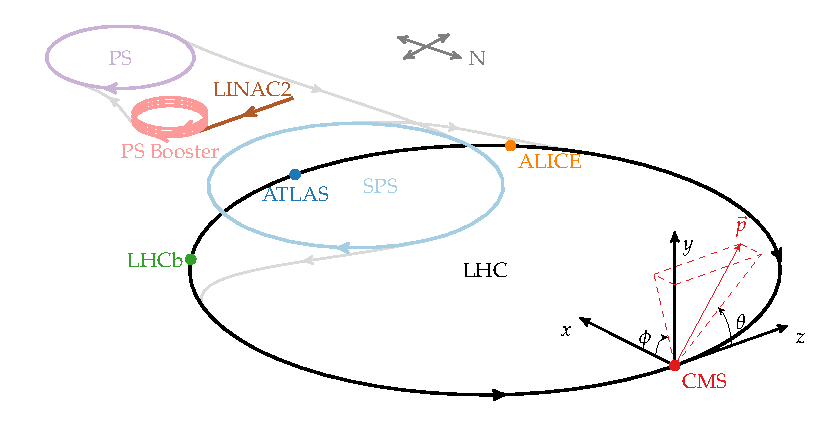
\includegraphics{diagrams/tikz/lhc_complex/lhc_complex.pdf}
    \caption{\cite{Mobs:2197559}}
    \label{fig:LHC-Complex}
\end{figure}

\subsection{\LHC Main Ring}

The main physics goals of the \LHC project was the discovery of the Higgs boson
and to observed new and rare \SM processes. The expected number of event rate of
a particular process with a cross section $\xs$ at a beam luminosity
$L$ is

\begin{equation}
    \mathcal{N} = L \xs \ .
\end{equation}

To increase the event rate the beam luminosity must increased. For Gaussian
beam distributions the luminosity can be given in terms of beam parameters as

\begin{equation}
    \label{eq:beam-lumi}
    L = \frac{N_b^2 n_b\frev\relgamma}{4\pi\emitt\bstar} F\ ,
\end{equation}

where $N_b$ is the number of particles per bunch, $n_b$ is the number of bunches
per beam, \frev is the revolution frequency, \relgamma is the relativistic gamma
factor, \emitt is the normalised transverse beam emittance, \bstar is the beta
function at the collision point (related to the transverse size of the beam) and
$F$ is the geometric luminosity reduction factor due to the crossing angle of
each beam at the crossing point.

At the \LHC, the luminosity is maximised by tuning all parameters in
Eq.~\eqref{eq:beam-lumi}. This necessitated the use of proton beams, circulating
in separate vacuum chambers and merging at insertion points to the detectors.
The beams nominally circulate in 2808 bunches with a spacing of ${\SI{25}{ns}}$
inside twin bore superconducting magnets --- two sets of coils and beam channels
within the same structure and cryostat --- achieving a peak dipole field of
${\SI{8.33}{T}}$ to bend the beam. Radio-frequency (RF) cavities apply the
potential gradient to accelerate the protons from ${\SI{450}{GeV}}$ to
${\SI{6.5}{TeV}}$. Quadrupole magnets focus the beam to suppress dispersion,
hence maintaining the beam luminosity. Additional quadrupoles focus the
beam as they enter the collision sections and defocus as they exit 
\cite{Bruning:782076}.

\section{Compact Muon Solenoid (\CMS) Experiment}

The conditions provided by the \LHC during 2016 data taking resulted in an
average number of collisions per bunch crossing of approximately 20, leading
to 1000 charged particles every ${\SI{25}{ns}}$ bunch crossing. The \CMS detector
was designed to account for particle multiplicities of this order by focusing on
high-granularity subdetectors with good time resolution. This requires a large
number of detector channels and millions of synchronised detector electronics, all
with a high radiation tolerance.

In addition to the conditions provided by the \LHC, the \CMS detector's design was
driven by four main physics requirements to achieve broad range of precision
measurements and new physics searches, namely: searching for the Higgs Boson,
supersymmetric particles, new massive vector bosons, extra dimensions; precision
studies of the \SM; and heavy-ion physics. The four requirements are summarised
as follows:

\begin{enumerate}
    \item \textbf{Muon identification:} ability to clearly
    identify muon up to $\aeta=2.5$ and dimuon mass resolutions of about $1\%$ for transverse momenta of \SI{100}{GeV}. The muon charge must be unambiguous up to
    muon momenta of \SI{1}{TeV}.
    \item \textbf{Charged particle reconstruction:} good momentum and reconstruction
    efficiency, particularly for the inner tracker, allowing for the identification
    of secondary vertices for the triggering and offline tagging $\tau$'s and
    $b$-jets. This requires a tracker component with a few cm of the interaction
    point.
    \item \textbf{Electromagnetic energy resolution:} measure the diphoton and
    dielectron mass with a resolution of $1\%$ for transverse momenta of
    \SI{100}{GeV} up to $\aeta=2.5$. Determine the direction of photons and the
    location of the primary interaction vertex. Efficiently reject \Ppizero decays
    into two photons and maintain prompt lepton isolation at high luminosities.
    \item \textbf{Transverse missing momentum and dijet mass resolution:} near
    complete reconstruction of the proton interaction to measure the transverse
    missing momentum. This requires a hermetic detector with hadron calorimeters
    extending up to $\aeta=5.0$ and fine component segmentation in the $\eta$-$\phi$
    plane of less than $0.1\times 0.1$.
\end{enumerate}

The full design of the \CMS detector for the 2016 data-taking period is shown in
Fig.~\ref{fig:cms-full} which achieves the requirements outlined above. The main
distinguishing feature of the \CMS detector is a ${\SI{3.8}{T}}$ superconducting
solenoid magnet enclosing the tracking and calorimetry subdetectors with and iron
return yoke to maintain a ${\SI{2}{T}}$ field outside the solenoid for the muon
subdetectors. All subdetectors are segmented into various regions in $\eta$ known
as the barrel (covering the central $\eta$ range) and endcap (covering up to
$\aeta=3.0$, with a slight overlap with the barrel). The hadronic calorimeter has an
additional segment in the forward region (covering $3<\aeta<5$) as required for
the missing momentum reconstruction. Further subdetector dependent segmentation is
done within the barrel, endcap and forward regions; discussed in further detail in
the following subsections. This gives the \CMS detector a total length of
${\SI{21.6}{m}}$ and a diameter of ${\SI{14.6}{m}}$ weighing ${\SI{12500}{tons}}$.

\begin{figure}[htbp]
    \centering
    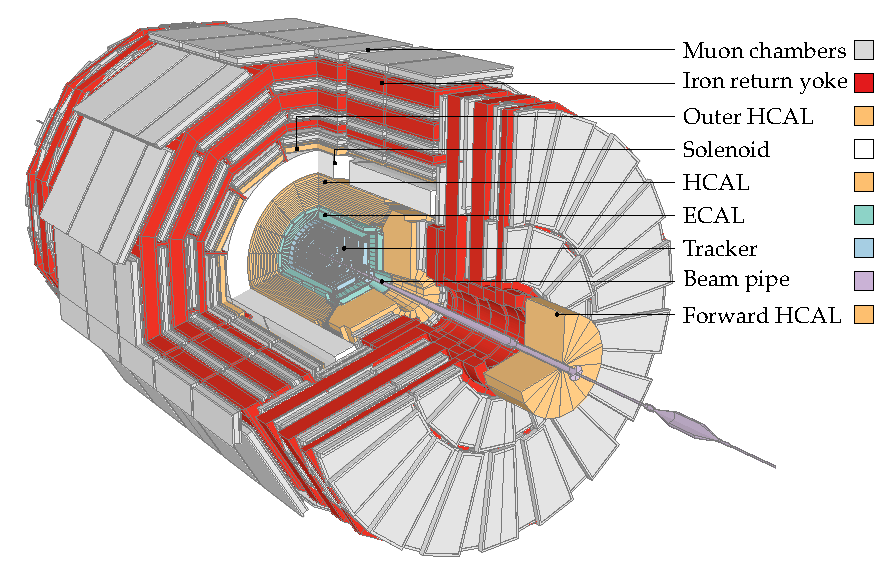
\includegraphics[]{diagrams/tikz/cms/annotated/cms_full.pdf}
    \caption{
        A schematic view of the \CMS detector and subdetectors during the 2016
        data-taking period, with a section removed to view the internal components.
        Acronyms are explained in the text. The diagram was produced using the tools
        outlined in \cite{Sakuma:2013jqa}.
    }
    \label{fig:cms-full}
\end{figure}

\subsection{Silicon Tracker}

The silicon tracker is the inner most subdetector to measure the position of charged
particles from ionisation deposits (known as hits) across a silicon-based
reverse-biased p-n junction for its for its high-granularity. A collection of hits
is used to reconstruct the curved path, with a radius of curvature $r$, of the
particle with a charge $q$ within the magnetic field $B$ to determine the momentum
of the particle transverse to the field, \pt, given by:

\begin{equation}
    \pt = rqB\ .
\end{equation}

A collection of tracks may intersect at a common point leading to the reconstruction
of the primary interaction, pileup and secondary vertices. These vertices are
typically a few centimetres apart, therefore, the tracker components are placed as
near as ${\SI{4.4}{cm}}$ from the beamline.

The silicon tracker, shown in Fig.~\ref{fig:cms-tracker}, consists of two main
components: silicon pixels and strips. The pixels measure 3-dimensional positional
coordinates of hits for environments of high particle flux (up to 10 million
particles per second), near the beam. Three layers of pixels are placed in the
barrel region (BPIX) at radii of ${\SI{4.4}{cm}}$, ${\SI{7.3}{cm}}$ and 
${\SI{10.2}{cm}}$ with a length of ${\SI{53}{cm}}$, centred on the z-axis. The pixel
models are staggered in the $\phi$-direction to achieve an overlapping
configuration. Additional pixels layers are placed in the endcap regions (FPIX) with
a turbine-like geometry with the blades rotated by ${\SI{20}{\degree}}$ for
overlapping blades. The overlap of pixel modules ensures the charged particle passes
through at least one module in each layer or blade. If two modules are hit the
charge sharing between these modules provides additional positional information on
the hit leading to improved position resolutions.

\begin{figure}[htbp]
    \centering
    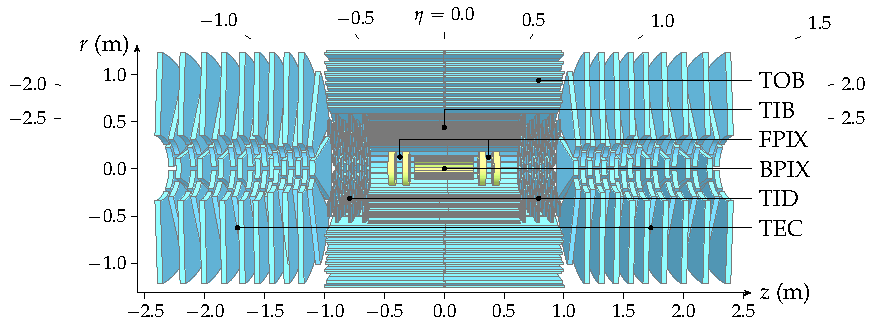
\includegraphics[]{diagrams/tikz/cms/annotated/cms_tracker.pdf}
    \caption{
        A cross-sectional view, in the $y$-$z$ plane, of the silicon tracker for the
        2016 data-taking period. The $r$, $z$ and $\eta$ dimensions of the detector 
        are shown. The acronyms used to label the various sub-components are defined
        in the text. The diagram was produced using the tools outlined in
        \cite{Sakuma:2013jqa}.
    }
    \label{fig:cms-tracker}
\end{figure}

Silicon strips are used further away from the beamline as the particle flux is
reduced. Strips provide an accurate 2-dimensional position for hits, hence layers
are typically oriented in a stereo-configuration for the full 3-dimensional
position. The silicon strips are separated into an inner and outer component. The
inner component is further split by the barrel and endcap regions. The tracker inner
barrel (TIB) component consists of 4 layers positioned at a radius of
${\SI{20}{cm}}$--${\SI{55}{cm}}$ and covering ${|z|<\SI{65}{cm}}$ with cell sizes of
${\SI{10}{cm}\times\SI{80}{\micro m}}$. The first 2 layers use the
stereo-configuration with an angle of ${\SI{100}{mrad}}$. The tracker outer barrel
(TOB) component has 6 layers extending the coverage to ${|z|<\SI{110}{cm}}$
and ${\SI{55}{cm}<r<\SI{130}{cm}}$. Again the first 2 layers are place in a
stereo-configuration with an angle of ${\SI{100}{mrad}}$. The inner endcap
(tracker inner disks, TID) component provides coverage for the gap between the
TIB and TOB with 3 small disks oriented perpendicular to the $z$-axis to avoid
excessive shallow track crossing angles. The first two disks have a
stereo-configuration. The tracker outer endcap (TEC) consists of 9 disks
extending into ${\SI{120}{cm}<|z|<\SI{280}{cm}}$ with stereo-configuration for
the first 2 and the fifth disks \cite{Borrello:687861}. The entirety of the silicon
detector comprises 66 million pixels and 9.6 million silicon strips with near
hermetic coverage up to $\aeta=2.4$.

To process all the data from the pixels and strips an on-detector chip processes
and buffers the analogue signal while waiting on a decision to accept or reject the
data. Upon an accept signal being received the data is transmitted over optical
links to off-detector chips for further processing, such as digitisation and data
formatting.

\subsection{\ECAL}

- Hermetic, homogenous calorimeter made of lead tung. divided into the barrel section (EB) and the endcap section comprising of the ECAL endcap (EE) and preshower (ES)
- Lead tungstate scintillating crystals have short radition (X0=0.89 cm) and Moliere (2.2 cm) lengths with fast responses (80\% of light emitted within 25 ns) and are radiation hard. However, low light yield (30 photons/MeV) require photodetectors with intrinsic gain that can operate in a magnetic field. Silicon avalanche photodiodes in the barrel and vacuum phototriodes in the endcaps.
- EB inner radius 129 cm with 36 supermodules each covering half the barrel length and aeta 0-1.479 and 20deg in phi. The crystals are titled at 3deg with respect to the nominal vertex position to avoid particles travelling fully inbetween two crystals. Crystal cover 0.0174 (1 deg) in phi and eta with front face cross-section of 22x22 mm**2 and length 230 mm -> 25.8 X0 (containment) and are contained in groups of 5 pairs within a thin-walled glass-fibre structure (submodules). Submodules are assembled into modules with 4 modules in each supermodule separated by aluminium webs
- EE 314cm from nominal vertex covering 1.479<aeta<3.0 structured as 2 dees - semi-circular aluminium plates with structural support units for 5x5 crystals (supercrystals). The crystals are rotated from the nominal vertex. Arranged in x-y grid. 28.6x28.6 mm**2 front face and a length of 220mm (24.7 X0). Special partial supercrystals cover the inner and outer circumference.
- ES only for endcap (1.653-2.6) for additional tracker space 2 planes of silicon strip detectors behind disks of lead absorbers at depths of 2X0 and 3X0 for pi0 rejection and provide directional information on the photon or electron.
- Readout: on-detector electronics ampplify and shape the signal from the sensors and digitise at 40 MHz. Data is buffered until an accept to transfer the data to off-detector electronics for further processing. The on-detector electronics also calculates trigger primitives transmitted at 40 MHz to the hardware trigger

- Corrections: E=G F sum(ci Ai)
G - global absolute scale determined in situ from Z->mumugamma. F - correction function depending on the type of particle, position, momentum and clustering algorithm (correct for energy loss from brem and containment variations from MC validated with a test beam and insitu with Z->ee and Z->mumugamma). ci - intercalibration coefficients with Ai - signal amplitudes (in ADC counts).
from light measurements  of crystal light yield, test beam precalibrations, cosmic rays, and in situ W->ev and pi0->gam gam and eta->gam gam mass reconstruction.
- Performance: supermodule measured in a test beam. Energy resolution (width containing 68\% of the energy) measured by fitting a gaussian function to the reconstructed energy distributions and parameterized as
...


The \ECAL is a homogeneous calorimeter made of lead tungstate (\pbwo) crystals
designed to provided calorimetric measurements of electromagnetic deposits
(typically electrons and photons) up to ${\aeta=3.0}$. The crystals have
short radiation lengths (${\SI{0.89}{cm}}$) and Moliere lengths
(${\SI{2.2}{cm}}$) allowing a compact design which absorbs a significant
portion of electromagnetic energy with a satisfactory level of radiation
resistance. The low light yield (${\SI{30}{photon/MeV}}$) from the crystals are
detected by photodetectors with intrinsic gain operable in the magnetic field.
Silicon avalanche photodiodes are used in the barrel and vacuum phototriodes in
the endcaps. Along with the barrel and endcaps, the \ECAL has a preshower system
installed in front of the endcaps for ${\Ppizero}$ rejection (since about
${98.8\%}$ of ${\Ppizero}$ decays into two photons with a very short lifetime,
${c\tau=\SI{25.5}{nm}}$). The preshower consists of two planes of silicon strip
detectors behind disks of lead absorber at depths of 2 and 3 radiation lengths.
The barrel covers a range of up to ${\aeta=1.479}$ with crystals of
${\SI{0.0174}{rad}}$ in \dphi and \deta and a length of ${\SI{230}{mm}}$ for
$25.8$ radiation lengths. The endcaps cover the region ${1.479<\aeta<3.0}$ in
an $x$-$y$ grid with a front cross section of ${28.6\times\SI{28.6}{mm^2}}$ and
a length of ${\SI{220}{mm}}$ (24.7 radiation lengths).

The energy resolution of the \ECAL is parameterised by

\begin{equation}
    \left(\frac{\sigma}{E}\right)^{2} = \left(\frac{S}{\sqrt{E}} \right)^{2}
    + \left( \frac{N}{E} \right)^{2} + C^2\ ,
\end{equation}

where $S$ is a stochastic tern, $N$ is a noise term and $C$ a constant term.
The total energy resolution ranges between {$1.50$--$0.35\%$} for
{$10$--$\SI{250}{GeV}$}, beyond which the constant term dominates.

\begin{figure}[htbp]
    \centering
    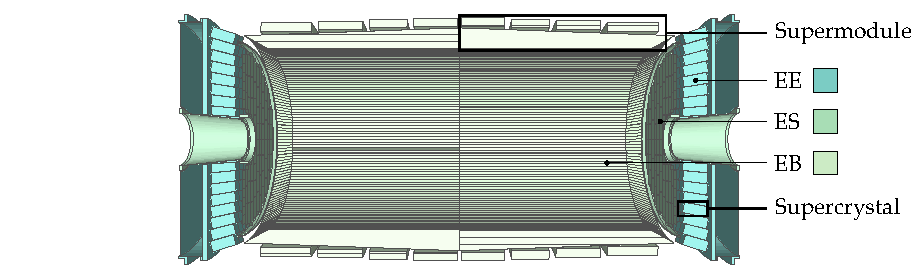
\includegraphics{diagrams/tikz/cms/annotated/cms_ecal.pdf}
    \label{fig:cms-ecal}
    \caption{
        A figure 
    }
\end{figure}

\subsection{\HCAL}

The \HCAL is designed to provide calorimetric measurements of hadronic activity
in an event. The barrel and endcap sections consist of brass/scintillator
sampling hadron calorimeters with coverage up to ${\aeta=3}$.

\begin{itemize}
    \item Brass/scintillator sampling hadron calorimeter with coverage up to
        ${\aeta=3.0}$. Scintillation detected by wavelength-shifting fibres
        embedded in the scintillator tiles and channeled to photodetectors
        via clear fibres. Then detected by hybrid photodetectors the provide
        gain and operate in high axial magnetic fields. Outer calorimeter
        in the iron return yoke beyond the magnet covering the barrel region
        adds about three interaction lengths ontop of the 8 provided by the
        inner calorimeter.
    \item Coverage up to ${\aeta=5.0}$ provided by iron/quartz-fibre
        calorimeter. Cerenkov light emitted by the quartz fibres is detected by
        photomultiplers. Ensure full coverage for the measurement of the
        transverse energy of an event.
\end{itemize}

\begin{figure}[htbp]
    \centering
    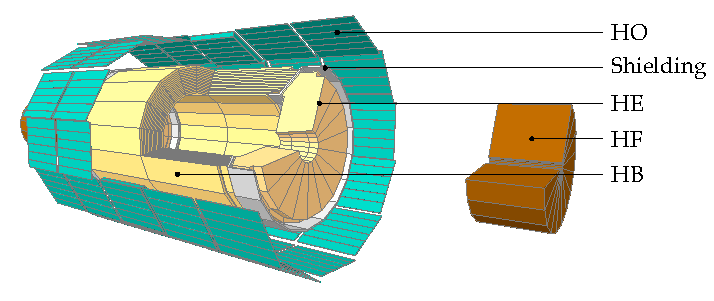
\includegraphics{diagrams/tikz/cms/annotated/cms_hcal.pdf}
    \label{fig:cms-hcal}
    \caption{
        A figure 
    }
\end{figure}

\subsection{Solenoid Magnet}

\begin{itemize}
    \item High-purity aluminium-stabilised conductor and indirect cooling (by
        thermosyphon).
    \item Bending power is designed around measuring muon momenta to a
        resolution of ${\Delta\mom/\mom\approx 10\%}$ at ${\mom = \SI{1}{TeV}}$.
    \item Favourable length/radius ratio chosen to ensure good momentum
        resolution in the forward region.
\end{itemize}

\begin{figure}[htbp]
    \centering
    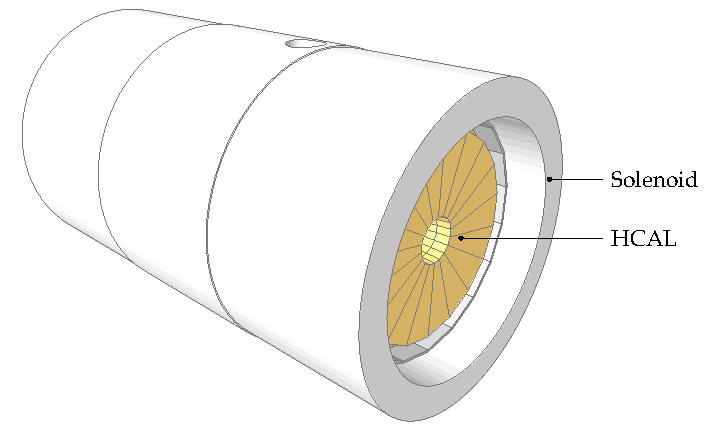
\includegraphics{diagrams/tikz/cms/annotated/cms_magnet.pdf}
    \label{fig:cms-magnet}
    \caption{
        A figure 
    }
\end{figure}

\subsection{Muon Chambers}

\begin{itemize}
    \item Resolution limited by multiple scattering in the central material
        up to $\pt=\SI{200}{GeV}$, when the chamber spatial resolution starts
        to dominate.
    \item Three types of gaseous deetctors.
    \item Barrel region (${\aeta<1.2}$), with low neutron induced background,
        the muon rate is low and residual field is low, drift tube chambers are
        used.
    \item 250 DT chambers in 4 layers. Staggered chambers allow high-\pt muons
        near boundaries to cross at least 3 out of the 4 layers. Each station is
        designed to give $\phi$ precision better and ${\SI{100}{\micro m}}$ in
        position and approximately ${\SI{1}{\milli rad}}$ in direction.
    \item The 2 endcaps, high muon and neutron induced background rate is high,
        and large field, cathode strip chambers are used to cover up to
        ${{\aeta}=2.4}$.
    \item 468 CSCs in 2 endcaps. Trapezoidal shape consisting of 6 gas gaps,
        each gap having radial cathode strips and a plane of anode wires running
        perpendicular to the strips. CSCs are overlapped in phi to avoid gaps
        in muon acceptance. Gas ionization and subsequent electron avalanche
        caused by charged particles produces a charge on the anode and image
        charge on the cathode. Precise precision measurement is made by
        determining the centre-of-gravity of the charge distribution induced on
        the cathode strips. Spatial resolution provided by each chamber from the
        strips is typically ${\SIrange{100}{200}{\micro m}}$ with an angular
        resolution in $\phi$ of the order of ${\SI{10}{\milli rad}}$.
    \item Resistive plate chambers are used in both regions. Operating
        in avalanche mode for good operation at high rates. Good timing
        resolution with coarse position resolution to identify the correct
        bunch crossing. Coverage up to ${\aeta<1.6}$ or ${\aeta<2.4}$.
\end{itemize}

\begin{figure}[htbp]
    \centering
    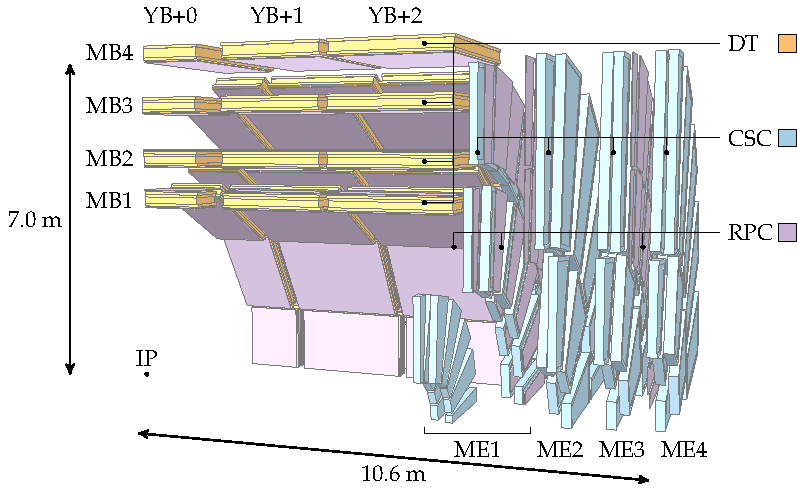
\includegraphics{diagrams/tikz/cms/annotated/cms_muons.pdf}
    \label{fig:cms-muons}
    \caption{
        A figure
    }
\end{figure}

    \begin{itemize}
        \item CMS 2006 detector TDR: \cite{Bayatian:922757}.
        \item CMS 2007 physics TDR: \cite{Bayatian:942733}.
        \item CMS 2005 computing TDR: \cite{Bayatyan:838359}.
        \item CMS 2000 TriDAS TDR: \cite{Bayatyan:706847}.
        \item CMS 2013 L1 trigger upgrade TDR: \cite{Tapper:1556311}.
        \item CMS 2012 HCAL upgrade TDR: \cite{Mans:1481837}.
        \item Luminosity report by CMS: \cite{CMS-PAS-LUM-17-001}.
    \end{itemize}

\subsection{Hardware Trigger}

\subsection{Software Trigger}

\subsection{Worldwide \LHC Computing Grid (\WLCG)}

%------------------------------------------------------------------------------%
